\documentclass{article}
\usepackage[utf8]{inputenc}
\usepackage[a4paper,scale={0.8,0.8}, marginratio={1:1}, bindingoffset=0mm]{geometry}
\usepackage{graphicx}
\usepackage{amsmath}
\usepackage{subcaption}	
\usepackage{float}
\usepackage[margin=\parindent,format=hang]{caption}
\usepackage{pdflscape}
\usepackage{multirow}
\usepackage[style=ieee, backend=bibtex]{biblatex}
\addbibresource{cite.bib}

\title{Evaluation of an Address Space\\ as a Means of Interaction with \\Internal State of Synchronized Sequential Logic}
\author{Matthijs Bos\\m.bos1@student.uva.nl\\Student nr. 10073558\\\\Supervisor:\\T. Walstra (UvA)\\ T.R.Walstra@uva.nl}

\begin{document}

\maketitle

\section{Introduction}

Previous work \cite{bos2016model} has presented a model for the application of field-programmable gate arrays (FPGA) as a tool for experimentation with digital logic. In this model, the concept of an address space has been adopted as a means of interaction with experiment setup logic. The address space serves as a primary means of interaction with an experiment setup, through the projection of experiment setup state on this address space. 

In the evaluation of this model however, the address space projections have been limited to experiment setup input and output signals. It has been suggested that the concept of an address space may also be suitable as a means of interaction with an experiment setup's elements of internal state, such as registers and memories. Although the model has been shown to support cycle-accurate control over experiment setups defined through synchronous sequential logic, interaction with stateful elements inside the experiment setup's logic is a significant objective in achieving practical applicability of the model. This article evaluates the capabilities of an address space as a means of interaction with an experiment setup's stateful elements within the context of the previously proposed model. 
% This evaluation is done on a number of different experiment setups defined through synchronous sequential logic. Existing implementations are adapted such that their elements of internal state are projected on the experiment setup's address space. 

% \subsection{Related Work}
% TODO

% \section{Address Space Projection}
% \label{section:projection}
% The model as proposed in \cite[Ch. 3]{bos2016model} has only provided an informal definition of the logic required for the projection of an experiment setup's signals on its address space. Additionally, this logic is currently being generated in an automated process, further concealing details on the process. As such, this section will first establish a formal model for the projection of experiment setup signals on an address space. This model is then extended to include the experiment setup's internal state elements in the process of address space projection. 

% \subsection{Experiment Setup Component}
% The experiment setup component as described in \cite[Sec. 3.4]{bos2016model} is defined to have an interface as displayed in figure \ref{fig:interface-experiment}. Both in terms of interface as well as behaviour, this component is defined to be similar to that of a block ram. As displayed in figure \ref{fig:timing-bram}, the \texttt{data out} output signal is defined to only change on positive clock edges. In terms of block rams, the experiment setup component is defined to operate in write-first mode, such that the signal for \texttt{data in} is always output during write operations.

% \begin{figure}
%     \centering
%     \caption{Experiment setup component interface. Copy of \cite[Fig. 3.11b]{bos2016model}.}
%     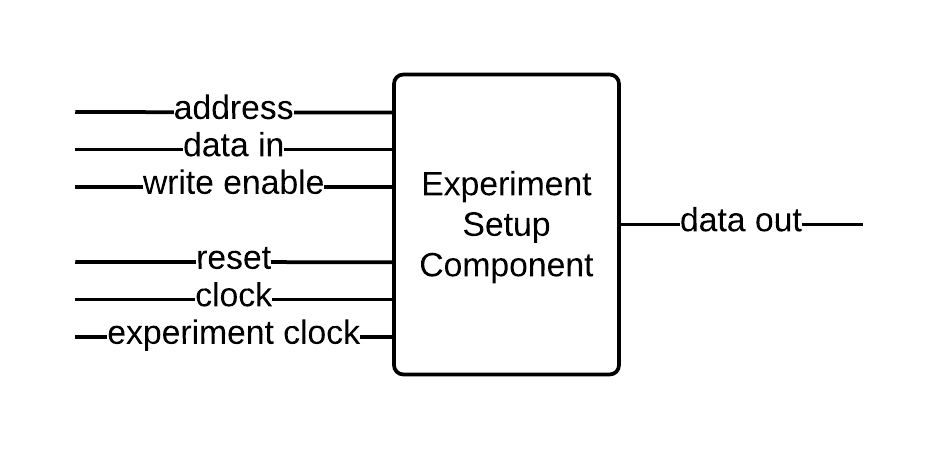
\includegraphics[width=0.5\textwidth]{img/interface-experiment.png}
% \label{fig:interface-experiment}
% \end{figure}

% \begin{figure}
%     \centering
%     \caption{Timing digram for experiment setup component. Copy of \cite[Fig. 3.12]{bos2016model}.}
%     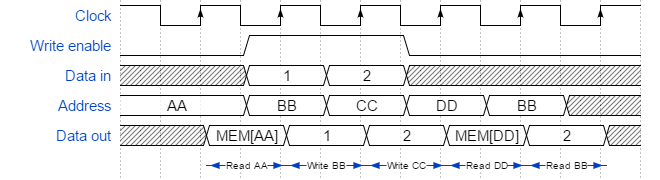
\includegraphics[width=0.8\textwidth]{img/timing-bram}
%     \label{fig:timing-bram}
% \end{figure}

% The widths for the experiment setup component's address and data buses are defined to correspond to the \texttt{address width} and \texttt{data width} parameters. The proposed model does not define specific widths for these signals and allows for these to be variable to suit different experiment setup scenarios.

% \subsection{Signal Projection}
% In the process of projecting experiment setup input and output signals onto an address space, one first defines a mapping between these signals and positions in the experiment setup's address space. Once a mapping between these signals is defined, one can define the logic that implements this mapping. 

% \subsection{Stateful Elements}
% Register, Memory, ROM, RAM, Register File

% Memory space defines a sequence of bits.

% Read interface
% - Asynchronous vs Synchronous read behaviour
% - 

% \begin{table}[]
% \centering
% \caption{My caption}
% \label{my-label}
% \begin{tabular}{lll}
% \textbf{Name} & \textbf{Direction} & \textbf{Width} \\
% \texttt{a}    & input              & 1              \\
% \texttt{b}    & input              & 13             \\
% \texttt{c}    & input              & 1              \\
% \texttt{x}    & output             & 1              \\
% \texttt{y}    & output             & 8              \\
% \texttt{z}    & output             & 24
% \end{tabular}
% \end{table}

% \begin{figure}
%     \centering
%     \caption{Caption}
%     \begin{align*}
%         \textbf{Address}& \rightarrow   \textbf{Signal}\\
%         0               & \rightarrow   \texttt{a} [0:0]\\
%         1               & \rightarrow   \texttt{b} [12:8]\\
%         2               & \rightarrow   \texttt{b} [7:0]\\
%         3               & \rightarrow   \texttt{c} [0:0]\\
%         4               & \rightarrow   \texttt{x} [0:0]\\
%         5               & \rightarrow   \texttt{y} [7:0]\\
%         6               & \rightarrow   \texttt{z} [23:16]\\
%         7               & \rightarrow   \texttt{z} [15:8]\\
%         8               & \rightarrow   \texttt{z} [7:0]
%     \end{align*}
%     \label{fig:my_label}
% \end{figure}

\newpage
\section{Exposing Internal Stateful Elements}

The nature of HDL modelling languages such as VHDL and Verilog HDL encourage the instantiation of design entities at lower levels of the design hierarchy, at the location where these are referenced and interconnected. As can be observed in figure \ref{fig:hierarchy-separate}, this habit of local instantiation results in a situation in which entities only contain references to lower-level instances. Additionally, an entity's interface signal definition must be satisfied on instantiation.

\subsection{Dependency Injection Principle}
\label{section:dip}
Application of the dependency injection principle is a common practice within the domain of object-oriented programming. A reference to the required components is passed to a lower-level object instance, such that instantiation can be transferred to a higher-level object instance. The dependency between two objects is often abstracted through the introduction of a separate interface definition. 

Hardware modelling languages such as VHDL and Verilog HDL do not offer a means for passing of instance references. A set of signal definitions can however be considered equal to an interface definition. The interconnection of two entities' signals can furthermore be considered equal to reference passing of an instance that implements a particular interface. Newer HDL modelling languages such as SystemVerilog natively include the concept of an interface as a means for the collective identification of a set of signals. Following the mapping between these concepts, the dependency injection principle can be considered applicable to the domain of HDL modelling, such that the instantiation of an entity instance can be transferred to a higher-level entity instance. Figure \ref{fig:hierarchy-di} provides a graphical display of the dependency injection principle. 

Since a signal's direction is of importance within the context of HDL modelling, the distinction between an interface and its complementary interface for consumption is made. In order to transfer the instantiation of a lower-level entity to a higher-level entity, the instantiating entity's definition is extended to include the inverse definition of the lower-level entity's. The lower-level entity is then instantiated in the higher-level entity and connected to its original parent.

\subsection{Dual-Interface Elements}
Application of the dependency inversion principle allows for the creation of design entities that are consumed by separate sibling entity instances. Figure \ref{fig:hierarchy-shared} displays an example design in which two entity instances consume a shared entity instance. Consumption of a shared instance allows for two logic components to share a common stateful element. 

As displayed in figure \ref{fig:hierarchy-semi-shared}, instantiation of a shared element does not necessarily have to happen in isolation. A dependency relationship between two entity instances can be established in order to allow for one to consume the other. By passing through one the signals, one can allow for interaction with a shared component that is instantiated locally, while reducing the amount of interfacing logic. 

As demonstrated in section \ref{section:implementation}, the application of the dependency injection principle as well as the creation of dual interface elements are important steps in the process of projection of stateful elements on the experiment setup's address space. The dependency injection principle is applied in order to isolate the stateful elements from the original experiment setup logic. This isolation then allows for these stateful elements to be converted to dual-interface elements, such that these allow to be interacted with through the experiment setup controller.


\begin{landscape}

\begin{figure}[]
    \centering%
    \caption{Illustration of the dependency injection principle applied to a hierarchy of entities in order to share a common instance.}
    \label{fig:hierarchy}
    \begin{subfigure}[t]{0.5\linewidth}
        \centering\captionsetup{width=0.95\linewidth}%
        \caption{Composition of entities in a hierarchical tree structure. The polygons represent different entity interfaces. An inverted polygon represents an interface's complementary definition for consumption.}
        \label{fig:hierarchy-separate}
        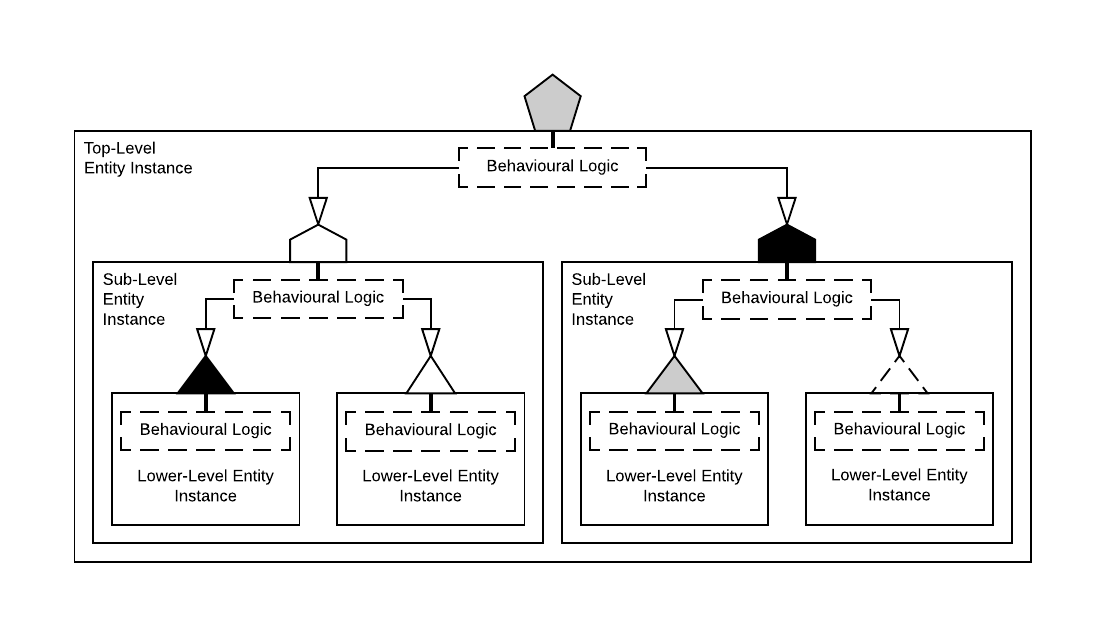
\includegraphics[width=0.95\textwidth,height=7cm,keepaspectratio,trim=70px 70px 70px 70px, clip=true]{img/hierarchy-separate}%
    \end{subfigure}%
    \begin{subfigure}[t]{0.5\linewidth}
        \centering\captionsetup{width=0.95\linewidth}%
        \caption{The dependency injection principle applied. The sub-level entity interfaces have been extended in order to allow for interconnection with lower-level entity instances that are instantiated in the top-level entity instance.}
        \label{fig:hierarchy-di}
        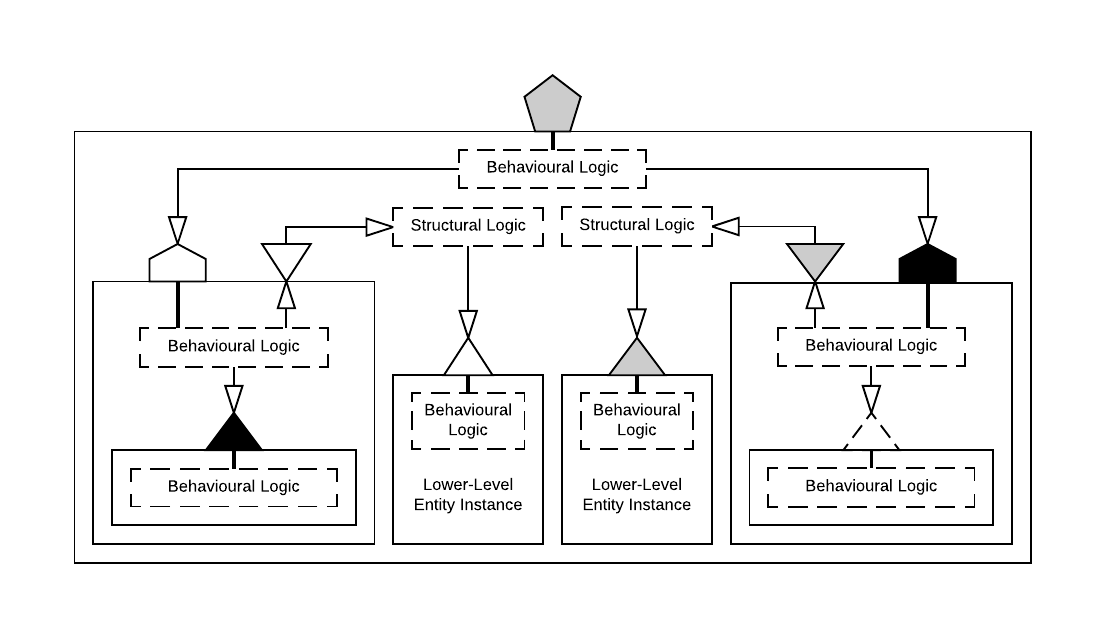
\includegraphics[width=0.95\textwidth,height=7cm,keepaspectratio,trim=70px 70px 70px 70px, clip=true]{img/hierarchy-di}%
    \end{subfigure}
    \begin{subfigure}[t]{0.5\linewidth}
        \centering\captionsetup{width=0.95\linewidth,belowskip=2em}%
        \caption{The application of the dependency injection principle allows for two branches in the instance hierarchy to share a common entity instance. This shared instance is instantiated in the top-level entity instance.}
        \label{fig:hierarchy-shared}
        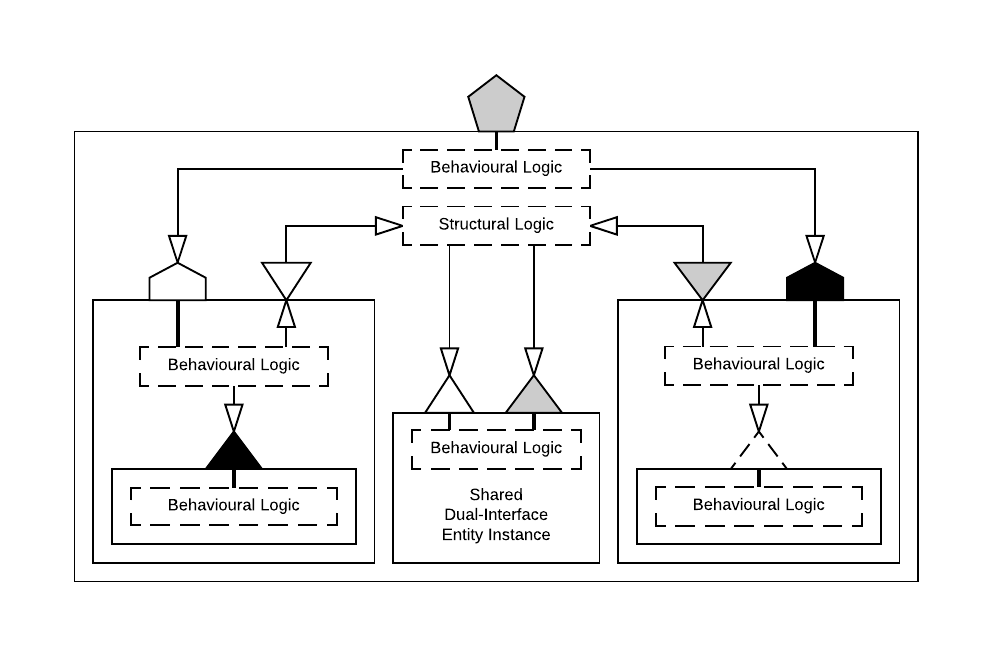
\includegraphics[width=0.95\textwidth,height=7cm,keepaspectratio,trim=70px 70px 70px 70px, clip=true]{img/hierarchy-shared}%
    \end{subfigure}%
    \begin{subfigure}[t]{0.5\linewidth}
        \centering\captionsetup{width=0.95\linewidth,belowskip=2em}%
        \caption{An alternative composition in which a shared entity is instantiated in a sub-level entity. The containing sub-level entity's interface has been extended to include a producer interface.}
        \label{fig:hierarchy-semi-shared}
        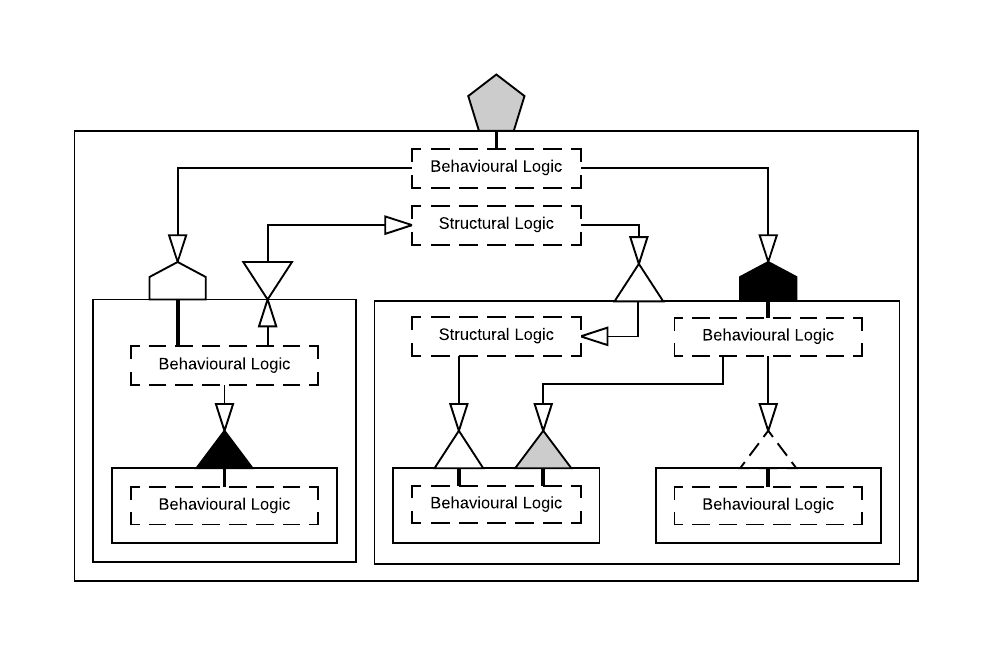
\includegraphics[width=0.95\textwidth,height=7cm,keepaspectratio,trim=70px 70px 70px 70px, clip=true]{img/hierarchy-semi-shared}%
    \end{subfigure}
\end{figure}

\end{landscape}

% \begin{figure}[h!]
%     \centering
%     \caption{Illustration of the dependency injection principle applied to a hierarchy of entities in order to isolate the stateful elements.}
%     \label{fig:hierarchy}
%     \begin{subfigure}[t]{0.5\textwidth}
%         \centering
%         \caption{Composition of entities in a hierarchical tree structure.}
%         \label{fig:hierarchy-default}
%         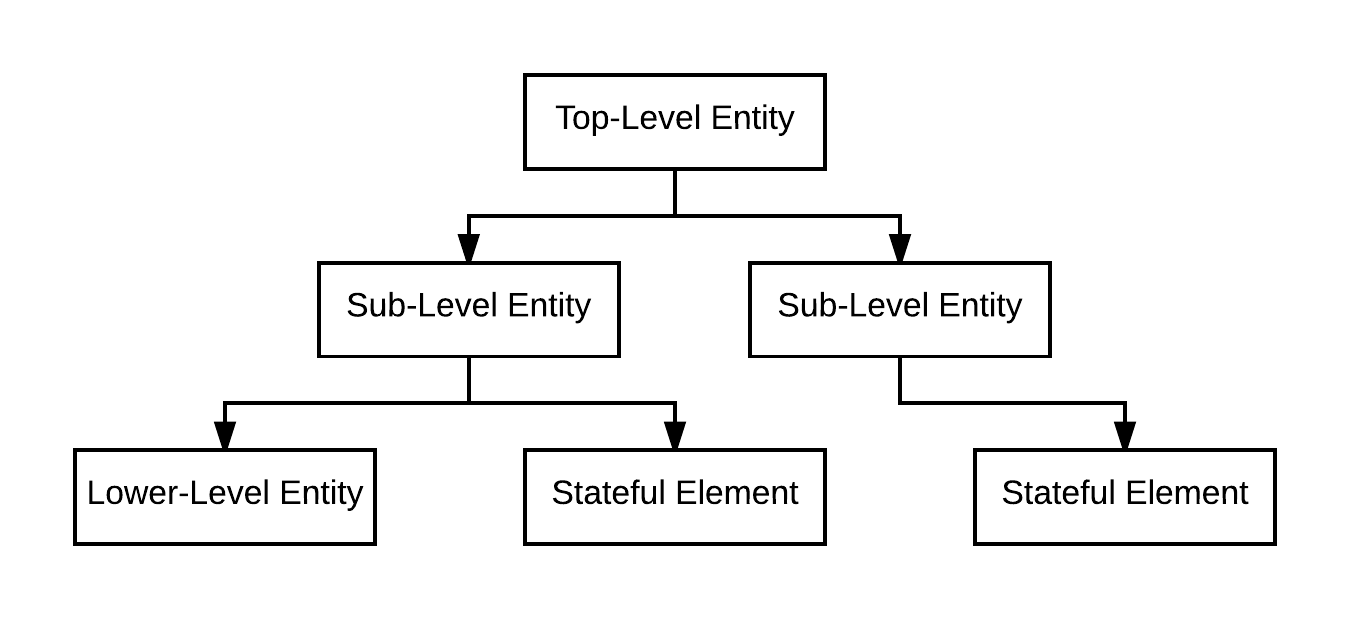
\includegraphics[width=\textwidth]{img/hierarchy-default}%
%     \end{subfigure}%
%     \begin{subfigure}[t]{0.5\textwidth}
%         \centering
%         \caption{The direct dependencies on the design's stateful elements have been inverted.}
%         \label{fig:hierarchy-inverted}
%         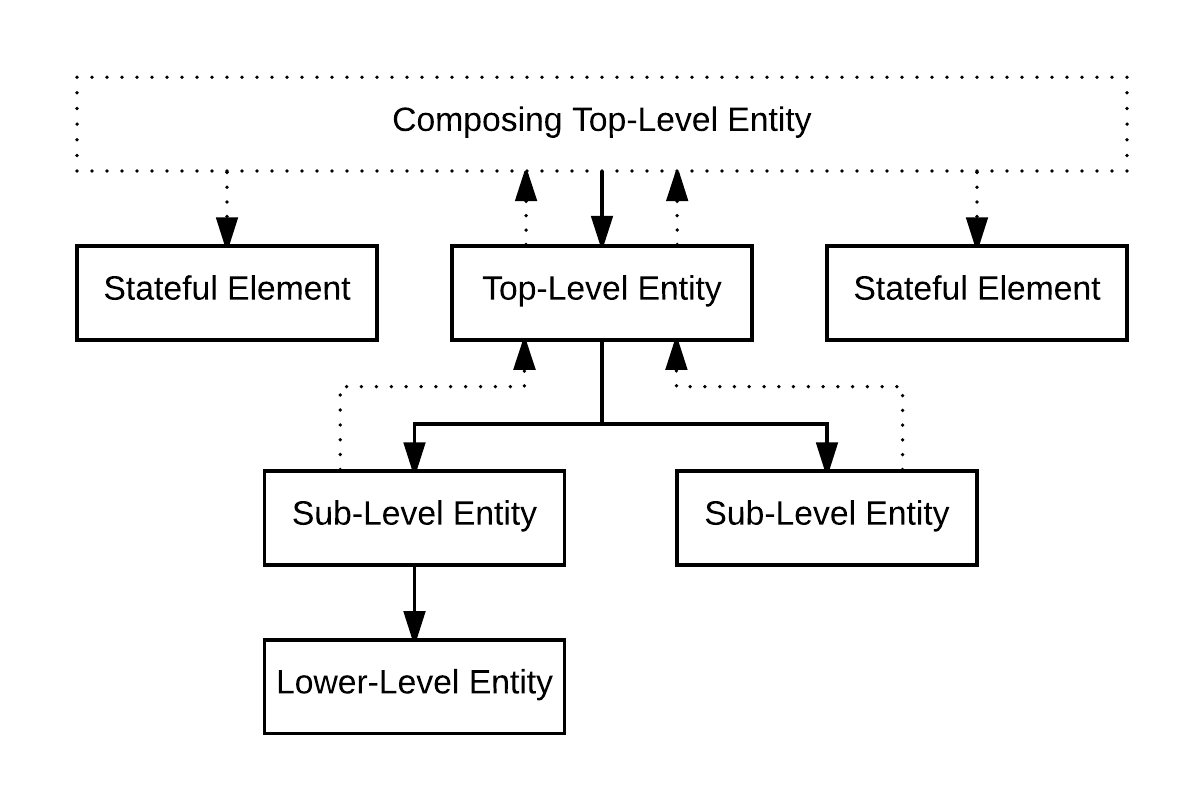
\includegraphics[width=\textwidth]{img/hierarchy-inverted}%
%     \end{subfigure}
% \end{figure}


% \begin{figure}[h!]
%     \centering
%     \caption{fig:stateful}
%     \label{fig:stateful}
%     \begin{subfigure}[t]{0.5\textwidth}
%         \centering
%         \caption{}
%         \label{fig:stateful-internal}
%         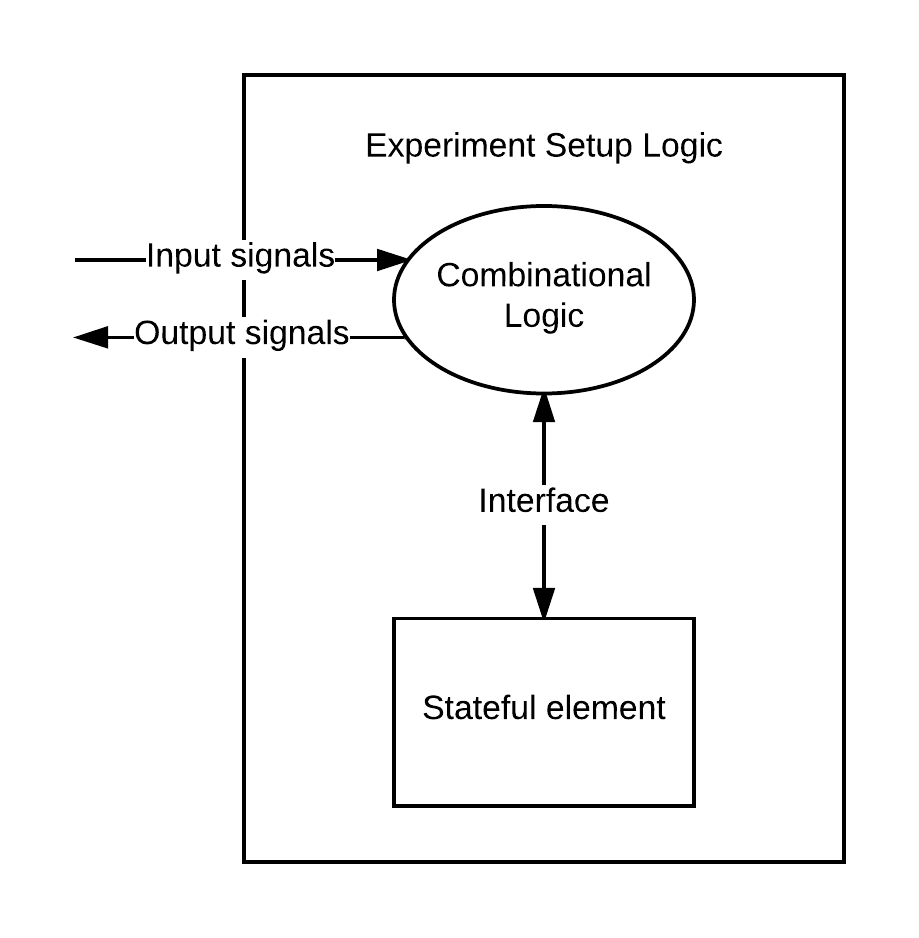
\includegraphics[width=\textwidth]{img/stateful-internal}%
%     \end{subfigure}%
%     \begin{subfigure}[t]{0.5\textwidth}
%         \centering
%         \caption{}
%         \label{fig:stateful-externalized}
%         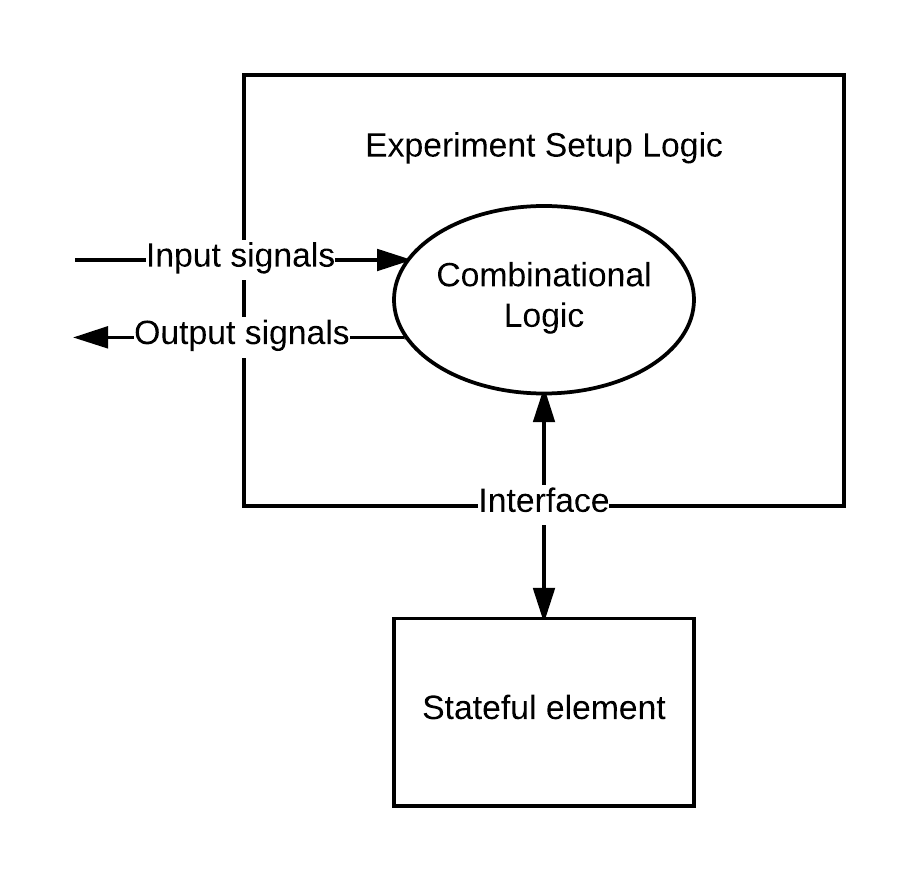
\includegraphics[width=\textwidth]{img/stateful-externalized}%
%     \end{subfigure}

% \end{figure}


\newpage
\section{Asynchronous Read Behaviour}
\label{section:async-read}
Experiment setup logic designs may contain elements of sequential logic which' read behaviour is defined to be asynchronous. One such example is the MIPS computer architecture as developed in \cite[Ch. 4]{hennessy2013computer}. For reading operations, all elements of sequential logic in this design are defined to reflect changes on their address bus without a clock signal triggering this change. Figures \ref{fig:async-read} and \ref{fig:async-read-timing} display a small design which emphasizes this type of behaviour.

\begin{figure}[h!]
    \centering
    \caption{An example logic design in which a ROM is defined to reflect changes on the address bus asynchronously. }
    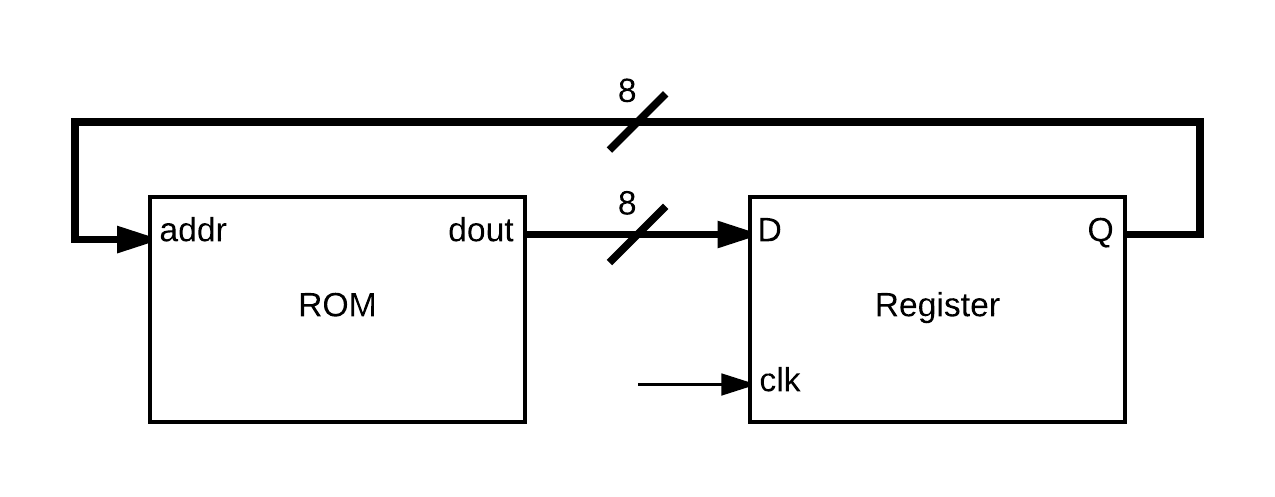
\includegraphics[width=0.7\textwidth]{img/async-read}
    \label{fig:async-read}
\end{figure}


\begin{figure}[h!]
    \centering
    \caption{Timing diagram displaying the behaviour for the logic elements displayed in figure \ref{fig:async-read}. The contents of the ROM are defined as such that $value(addr) = addr + 1$. The ROM's propagation delay is identified by \texttt{t\textsubscript{delay}}.}
    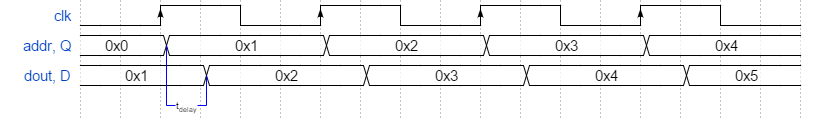
\includegraphics[width=\textwidth]{img/mem-async}
    \label{fig:async-read-timing}
\end{figure}


Projecting this immediate read behaviour on a FPGA proves to be problematic in the case of large memories. Small stateful elements, such as registers or register files can be translated to CLB flip-flops, allowing for preservation of the asynchronous read behaviour. Large memory elements however, are generally projected on a FPGA's block ram elements which' read and write behaviour is synchronous, requiring one or more clock cycles to complete its operations. A design requiring even larger memories may make use of the FPGA's peripheral memory devices, such as SRAM or DRAM ICs. These peripheral devices generally introduce significant latencies for reading and writing operations. 

\subsection{Clock Delay}
\label{section:clock-delay}
Through intentional delay of the experiment setup clock, these relatively slow memory devices can still be utilized to behave asynchronously. The experiment setup logic clock signal can be considered a subsample of the global clock signal. More specifically, this signal operates at irregular intervals between global clock pulses. Through operation of the slow memory devices off the global clock signal, the idle time in-between experiment setup clock cycles allow for these synchronous elements to update their data outputs and expose asynchronous read behaviour from the perspective of the experiment setup logic.

One could compare this type of behaviour to a situation of two clock domains in which a high-latency memory element operating at high frequency is consumed by another component operating at a relatively lower frequency. The current approach avoids challenges related to clock domain crossing however, since both clocks are defined to be similar, except for the fact that the experiment setup's clock signal is occasionally disabled. 

% Figures \ref{fig:async-read-rom} and \ref{fig:mem-async-exp-clk} 

\begin{figure}[h!]
    \centering
    \caption{Example logic design similar to figure \ref{fig:async-read} that features a synchronous \texttt{ROM}, requiring a clock input. The triangle represents a clock gating buffer that is controlled by the \texttt{exp\_clk\_en} signal.}
    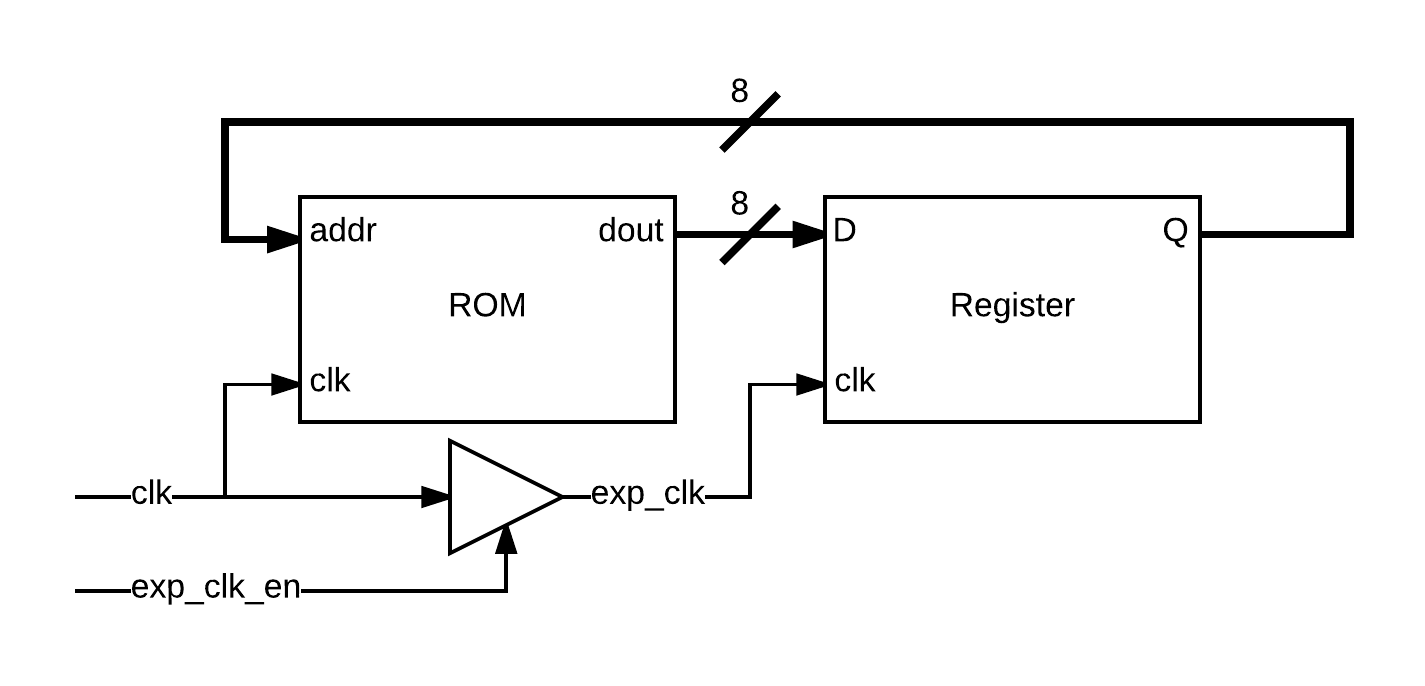
\includegraphics[width=0.7\textwidth]{img/async-read-rom}
    \label{fig:async-read-rom}
\end{figure}

\begin{figure}[h!]
    \centering
    \caption{Timing diagram displaying the behaviour for the logic elements displayed in figure \ref{fig:async-read-rom}. The blue curved line follows a sequence of events that show how the signal changes propagate.}
    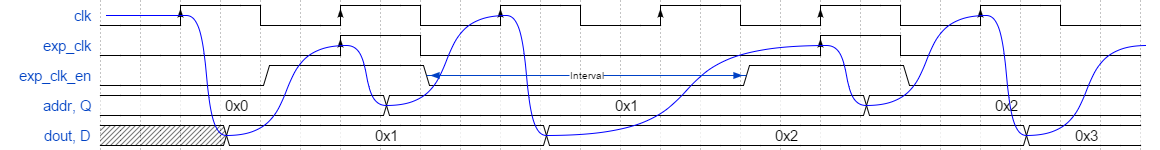
\includegraphics[width=\textwidth]{img/mem-async-exp-clk}
    \label{fig:mem-async-exp-clk}
\end{figure}

\subsection{Synchronous Write}
A consequence of a memory element operating off the continuous global clock signal is that write operations are synchronized with this signal as well. Write operations are generally triggered trough a pulse on a write enable signal. Since the write enable signal is controlled through experiment setup logic, this pulse may span multiple global clock cycles, triggering multiple write operations.  

In order for a write operation to be executed only once on the experiment setup clock signal's rising edge, additional logic is required. Figure \ref{fig:async-read-ram} displays an example RAM which operates off the global clock signal. An and-gate is included to prevent the RAM's write enable signal \texttt{wen} to be raised unless an experiment setup clock cycle is executed. This is achieved trough conjunction of the experiment setup's \texttt{wen} signal and the \texttt{exp\_clk\_en} signal. As displayed in figure \ref{fig:mem-async-exp-clk}, the \texttt{exp\_clk\_en} is raised before the experiment setup clock signal's rising edge occurs. 

\begin{figure}[h!]
    \centering
    \caption{Example logic design in which additional logic is included to prevent the the RAM's \texttt{wen} signal to be raised in-between experiment setup clock cycles.}
    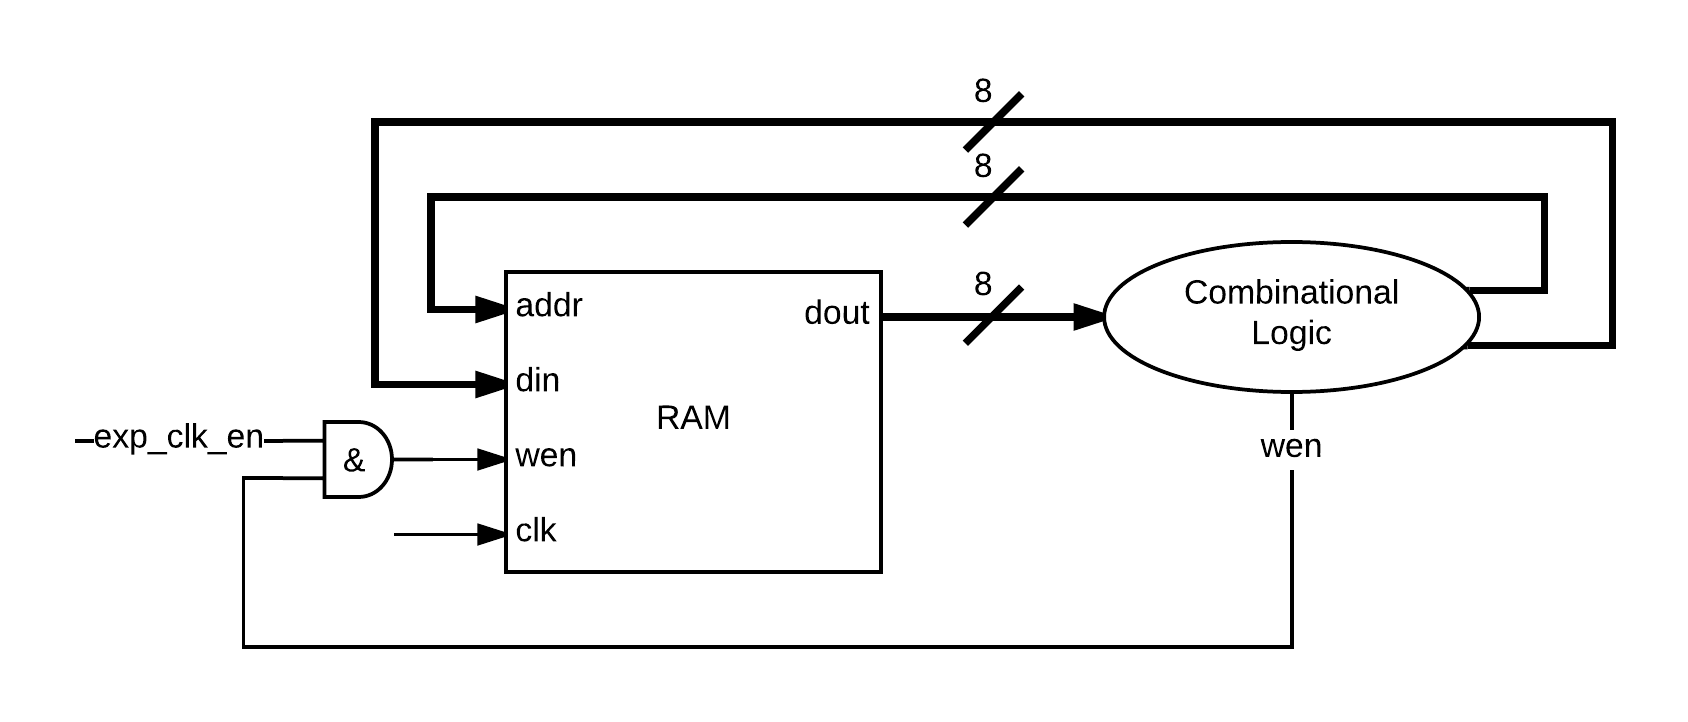
\includegraphics[width=0.7\textwidth,trim=70px 70px 70px 70px, clip=true]{img/async-read-ram}
    \label{fig:async-read-ram}
\end{figure}


\newpage
\section{Implementation}
\label{section:implementation}
An existing MIPS implementation has been modified to support interaction through an address space. More specifically, this implementation features an implementation of a simple single-cycle MIPS computer architecture, very similar to the design developed in \cite[Sec. 4.4]{hennessy2013computer}. Although limited in the number of supported instructions, the implementation follows the instruction format specification as established in \cite[Ch. 2]{hennessy2013computer}. Source code for the original version\footnote{\url{https://github.com/tcamolesi/simple-mips}} as well as this article's modified version\footnote{\url{https://github.com/matthijsbos/simple-mips-fpgaedu}} are publicly available on GitHub. This article's implementation is targeted at a Digilent Nexys 4 FPGA development board, featuring a Xilinx Artix-7 FPGA. The Xilinx Vivado IDE has been used for compilation of HDL sources.


\subsection{Types of Stateful Elements}

Although limited in terms of complexity and optimizations, the single-cycle MIPS design makes use of a variety of types of stateful elements, making it suitable as a means for establishing a proof of concept for the theory introduced in section \ref{section:projection}. Although optimizations such as pipelining introduce additional stateful elements into the design, these elements do not contribute to an increased variation of stateful elements types, since primitive registers can be used for this purpose. 

\begin{itemize}
    \item A 32-bit register is used as a program counter.
    \item The register file features a combination of immediate read behaviour as well as synchronous write behaviour.
    \item The instruction memory is defined to provide immediate read behaviour.
    \item The data memory is defined to provide immediate read behaviour while allowing for synchronous write operations. 
\end{itemize}

\subsection{Externalization of Stateful Elements}

Applying the model as described in \cite{bos2016model} results in a hierarchical design as displayed in figure \ref{fig:mips-original} in which the stateful elements are instantiated locally. In order to project these elements on the experiment setup's address space, these need to be isolated and wrapped such that a dual-interface element is created. This is achieved through application of the dependency injection principle as described in section \ref{section:dip}. Figure \ref{fig:mips-wrapped} displays the result of this process. Instantiation of the MIPS' internal stateful elements has been delegated to a higher-level entity and these have been wrapped such that a dual-interface component is created. The introduction of a dual-interface element allows for the stateful element to be consumed by the MIPS implementation as well as the experiment setup controller. 

\begin{figure}
    \centering
    \caption{Hierarchical composition of single-cycle MIPS implementation. The MIPS' internal stateful elements are instantiated locally.}
    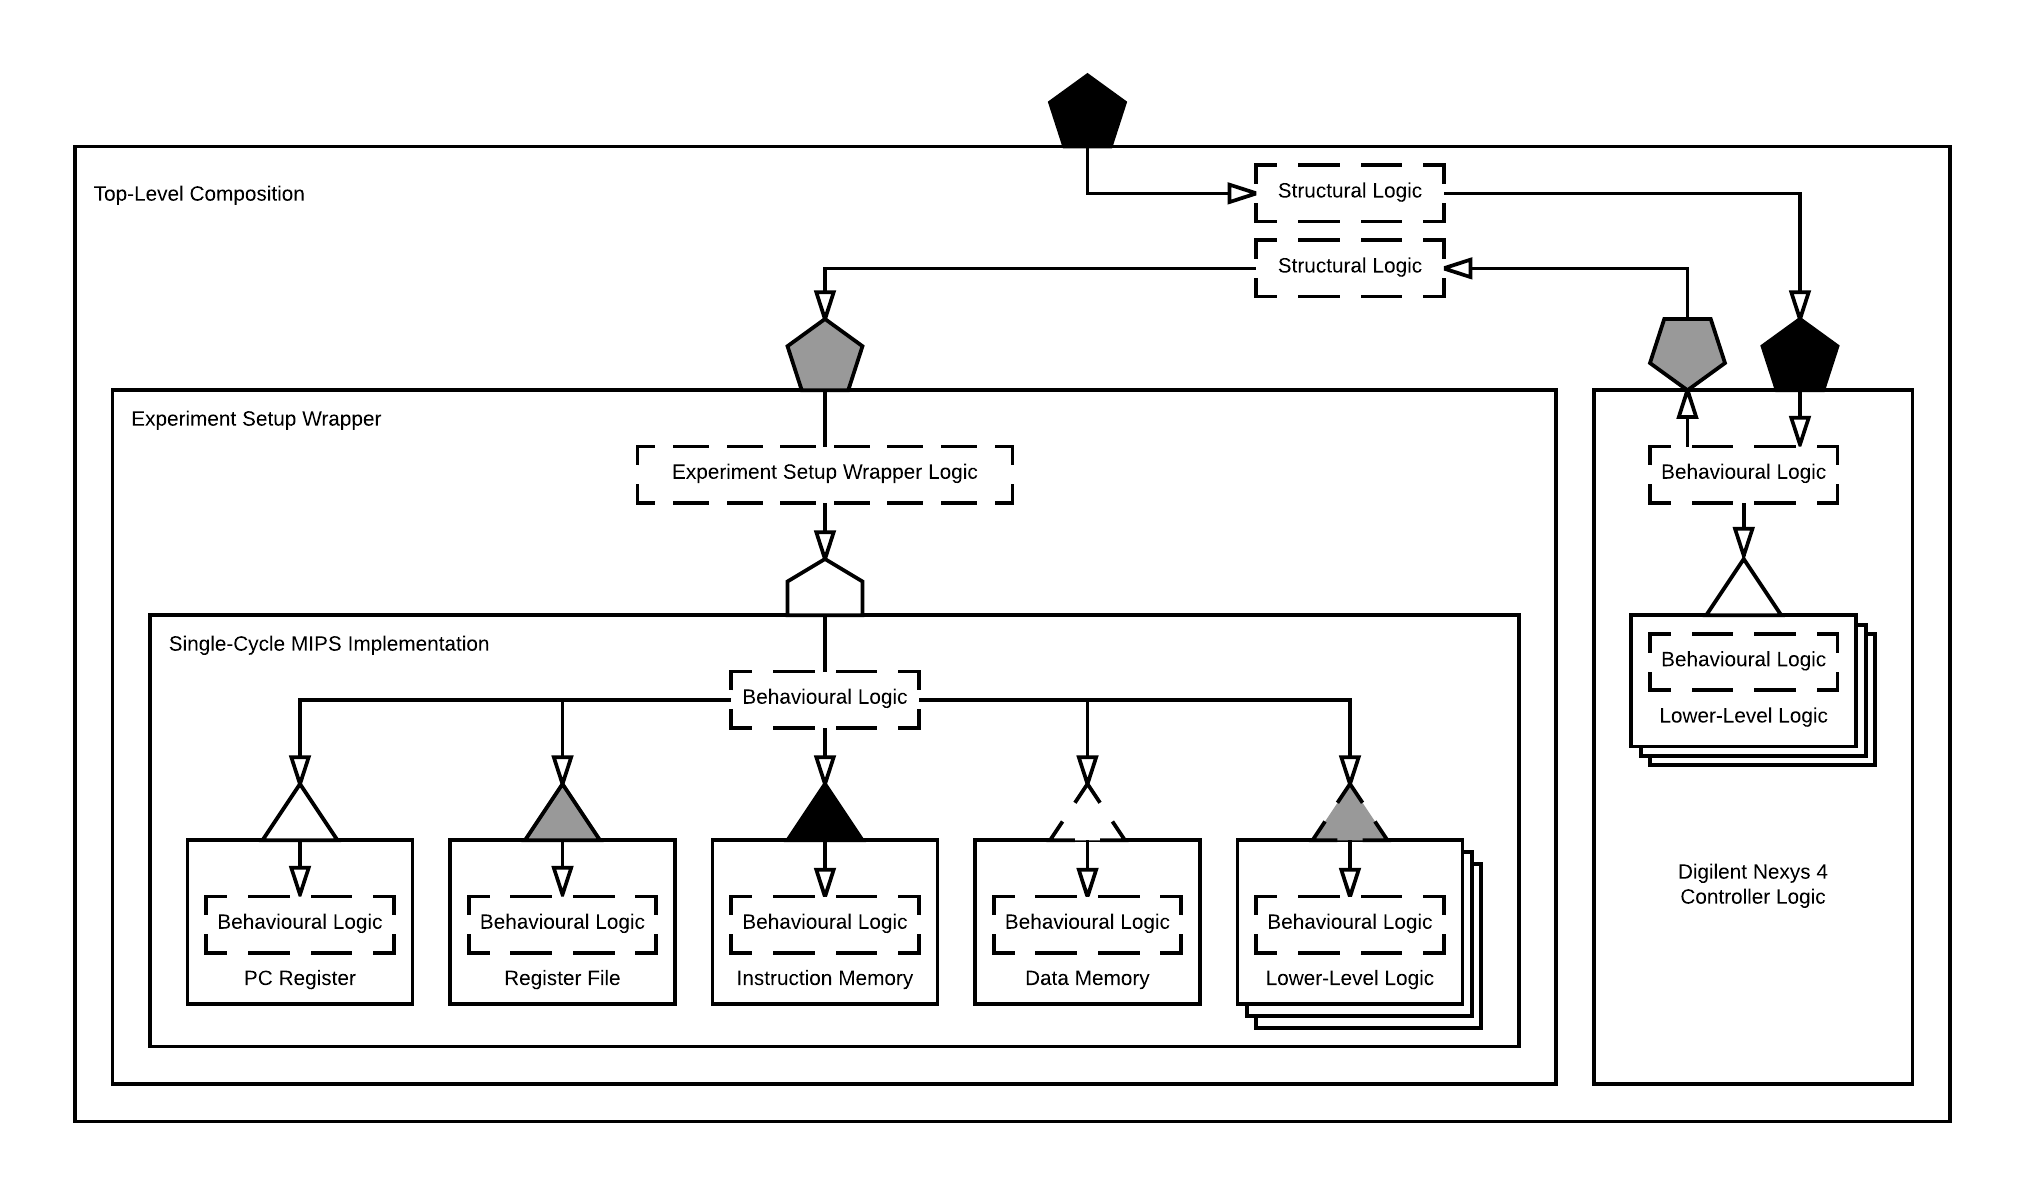
\includegraphics[width=\textwidth,trim=70px 70px 70px 70px, clip=true]{img/mips-original}
    \label{fig:mips-original}
\end{figure}

For the purpose of this implementation, the FPGA's internal block RAM elements have been utilized for the implementation of the instruction memory as well as the data memory. Both memory elements have been set to contain 1024 elements of 32-bit data words, resulting in bus widths of 10 and 32 for the address and data buses respectively. Although the size of these memories is relatively small, these suit the purpose of the proof of concept. Any memory size can be selected, as long as the FPGA's memory resources can accommodate the requirements. 

Like FPGAs from other manufacturers, Xilinx 7 Series FPGAs come equipped with dual-port block RAM elements. The presence of this type of functionality eases the process of creating dual-interface stateful elements. Instead of adding additional logic for the multiplexing of the consuming interface, the FPGA provides this functionality natively. The theory introduced in section \ref{section:async-read} has been applied to the wrapping logic in order to allow for both memories to expose asynchronous read behaviour.

An early design decision has been to extend the original experiment setup component interface to include the \texttt{exp\_clk\_en} signal, such that this signal's level can be used to select between the consuming component. This addition is of particular relevance for the handling of write operations. As can be observed in the timing diagram displayed in figure \ref{fig:mem-async-exp-clk}, the \texttt{exp\_clk\_en} signal is raised during an entire experiment setup clock cycle, indicating an upcoming rising edge on the experiment setup clock. The interface displayed in figure \ref{fig:interface-experiment-setup-component} includes the additional input signal.

Although the instruction memory solely offers read-only functionality to the MIPS implementation, a fully-featured RAM element has been used to implement this behaviour. This decision has allowed for modification of the instruction memory's contents through the address space projection. Being unable to modify the ROM's contents at runtime would limit the capability of setting the instruction memory's contents at compile time during bitstream generation.

Utilization of the FPGAs built-in memory resources for the MIPS' memories forces a clean separation between the stateful component and the wrapping logic. The wrapper implementation for the MIPS' register components however, has allowed for a more integral approach in which the original components have been extended to include an interface for interaction through an address space. 


\begin{figure}
    \centering%
    \caption{Interface defintions for those displayed in figures \ref{fig:mips-original} and \ref{fig:mips-wrapped}.}
    \label{fig:interfaces}
    \begin{subfigure}[b]{0.33\linewidth}
        \centering\captionsetup{width=0.95\linewidth}%
        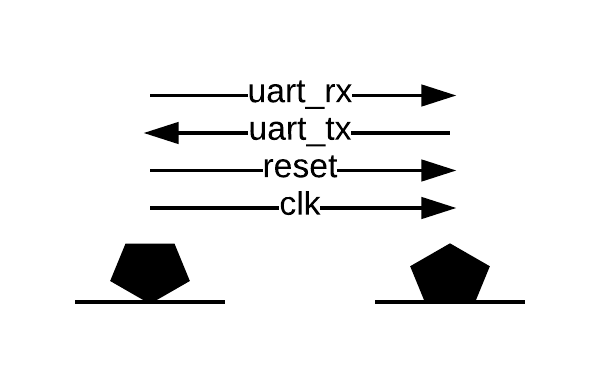
\includegraphics[width=0.70\textwidth,trim=70px 70px 70px 70px, clip=true]{img/interface-nexys4}%
        \caption{Nexys 4 controller}
    \end{subfigure}%
    \begin{subfigure}[b]{0.33\linewidth}
        \centering\captionsetup{width=0.95\linewidth}%
        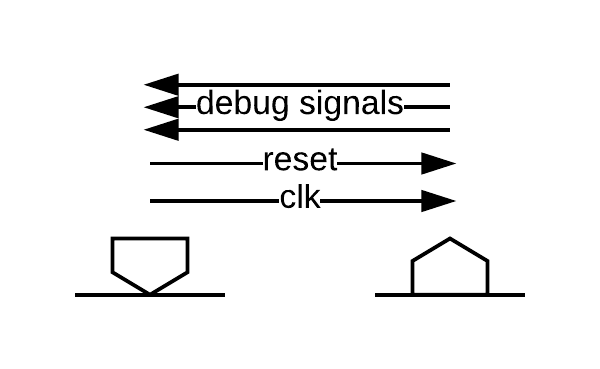
\includegraphics[width=0.70\textwidth,trim=70px 70px 70px 70px, clip=true]{img/interface-mips}%
        \caption{Single-cycle MIPS}
    \end{subfigure}%
    \begin{subfigure}[b]{0.33\linewidth}
        \centering\captionsetup{width=0.95\linewidth}%
        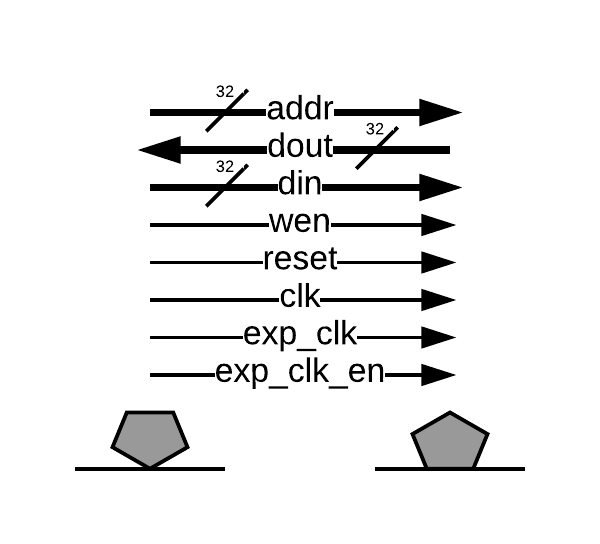
\includegraphics[width=0.70\textwidth,trim=70px 70px 70px 70px, clip=true]{img/interface-experiment-setup-component}%
        \caption{Experiment setup component}
        \label{fig:interface-experiment-setup-component}
    \end{subfigure}
    
    \begin{subfigure}[b]{0.25\linewidth}
        \centering\captionsetup{width=0.95\linewidth}%
        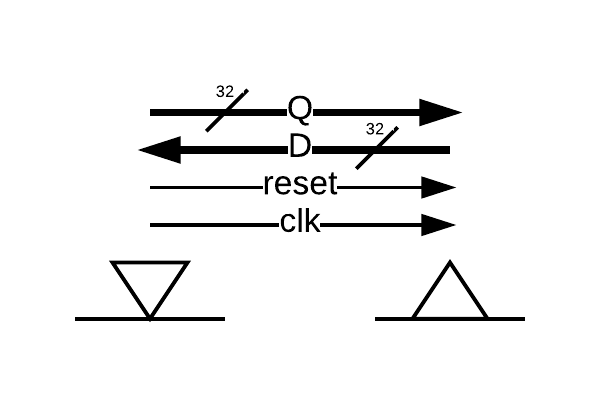
\includegraphics[width=0.95\textwidth,trim=70px 70px 70px 70px, clip=true]{img/interface-register}%
        \caption{PC register}
    \end{subfigure}%
    \begin{subfigure}[b]{0.25\linewidth}
        \centering\captionsetup{width=0.95\linewidth}%
        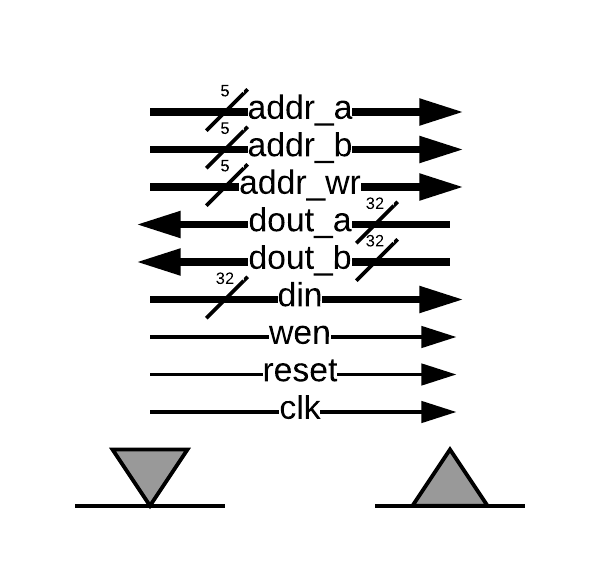
\includegraphics[width=0.95\textwidth,trim=70px 70px 70px 70px, clip=true]{img/interface-register-file}%
        \caption{Register file}
    \end{subfigure}%
    \begin{subfigure}[b]{0.25\linewidth}
        \centering\captionsetup{width=0.95\linewidth}%
        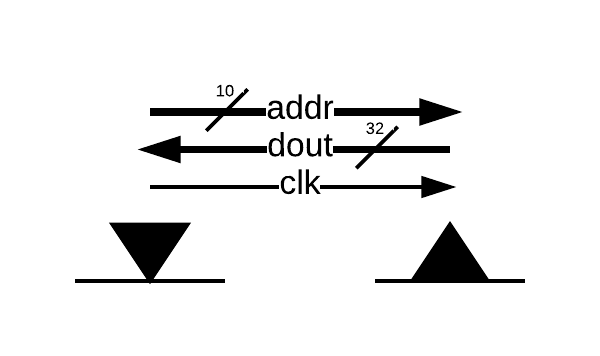
\includegraphics[width=0.95\textwidth,trim=70px 70px 70px 70px, clip=true]{img/interface-rom}%
        \caption{Instruction memory}
    \end{subfigure}%
    \begin{subfigure}[b]{0.25\linewidth}
        \centering\captionsetup{width=0.95\linewidth}%
        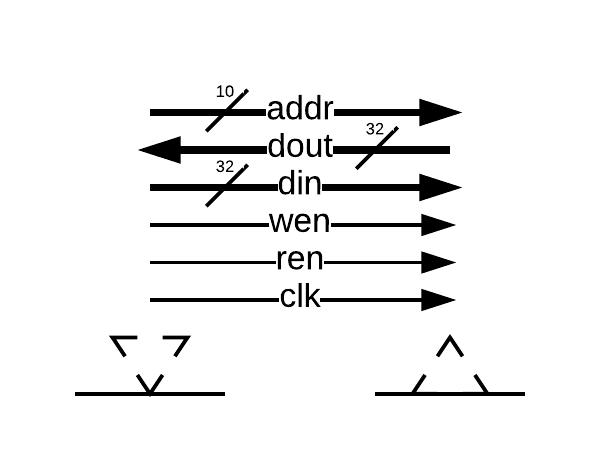
\includegraphics[width=0.95\textwidth,trim=70px 70px 70px 70px, clip=true]{img/interface-ram}%
        \caption{Data memory}
    \end{subfigure}%

\end{figure}

\subsection{Address Space Unification}
The externalization and wrapping of the separate stateful elements creates separate 'miniature' experiment setups with their own address space and corresponding interface. Additional logic is required in order for these separate components to be projected on a single address space. As can be observed in figure \ref{fig:mips-wrapped}, address space partitioning logic is added to the design that interconnects the different wrapper instances. 

In the current design, a single implementation of a binary address space partitioning element is used. This element is used to select between two child experiment setup components based on the address value on the master address bus as provided by the controller. The component is parametrized such that the address ranges for both partitions can be set. An additional parameter is provided for both child experiment setup components that subtracts a given value from the master bus' address. This feature allows for an address in the global address space to be translated to an address in a local address space. 

In this article's implementation, four instances of this binary component have been daisy-chained together in order to allow for five local address spaces to be projected on the experiment setup's global address space. Table \ref{tbl:address-space} provides a detailed description of the resulting address space. These four paritioning elements could have been replaced by a single design entity to reduce the amount of logic elements and interconnections. For the purpose of simplicity and extensibility however, the current approach has been taken. 


% Please add the following required packages to your document preamble:
% \usepackage{multirow}
\begin{table}[]
\centering
\caption{An description of the experiment setup's unified address space. The different local address spaces have been projected on five partitions.}
\label{tbl:address-space}
\begin{tabular}{|l|r|l|r|r|l|}
\hline
\multicolumn{2}{|c|}{\textbf{Partition}}                     & \multicolumn{4}{c|}{\textbf{Signal}}                                                     \\ \hline
\textbf{Description}                & \textbf{Addr. Offset}  & \textbf{Description} & \textbf{Addr. Offset} & \textbf{Abs. Addr.} & \textbf{Read/Write} \\ \hline
\multirow{18}{*}{MIPS Debug}        & \multirow{18}{*}{0}    & PC                   & 0                     & 0                   & Read-only           \\ \cline{3-6} 
                                    &                        & PC next              & 1                     & 1                   & Read-only           \\ \cline{3-6} 
                                    &                        & Opcode               & 2                     & 2                   & Read-only           \\ \cline{3-6} 
                                    &                        & RS addr              & 3                     & 3                   & Read-only           \\ \cline{3-6} 
                                    &                        & RT addr              & 4                     & 4                   & Read-only           \\ \cline{3-6} 
                                    &                        & RD addr              & 5                     & 5                   & Read-only           \\ \cline{3-6} 
                                    &                        & Funct                & 6                     & 6                   & Read-only           \\ \cline{3-6} 
                                    &                        & Immed                & 7                     & 7                   & Read-only           \\ \cline{3-6} 
                                    &                        & Reg q0               & 8                     & 8                   & Read-only           \\ \cline{3-6} 
                                    &                        & Reg q1               & 9                     & 9                   & Read-only           \\ \cline{3-6} 
                                    &                        & Reg wdata            & 10                    & 10                  & Read-only           \\ \cline{3-6} 
                                    &                        & Instr data           & 11                    & 11                  & Read-only           \\ \cline{3-6} 
                                    &                        & Instr. addr          & 12                    & 12                  & Read-only           \\ \cline{3-6} 
                                    &                        & Data mem wen         & 13                    & 13                  & Read-only           \\ \cline{3-6} 
                                    &                        & Data mem ren         & 14                    & 14                  & Read-only           \\ \cline{3-6} 
                                    &                        & Data mem wdata       & 15                    & 15                  & Read-only           \\ \cline{3-6} 
                                    &                        & Data mem addr        & 16                    & 16                  & Read-only           \\ \cline{3-6} 
                                    &                        & Data mem rdata       & 17                    & 17                  & Read-only           \\ \hline
Program Counter                     & 99                     & PC Register          & 0                     & 99                  & Read+Write          \\ \hline
\multirow{3}{*}{Register File}      & \multirow{3}{*}{100}   & Register 0, \$zero   & 0                     & 100                 & Read+Write          \\ \cline{3-6} 
                                    &                        & \multicolumn{4}{c|}{\vdots}                                                              \\ \cline{3-6} 
                                    &                        & Register 31, \$ra    & 31                    & 131                 & Read+Write          \\ \hline
\multirow{3}{*}{Instruction Memory} & \multirow{3}{*}{10000} & Instruction 0        & 0                     & 10000               & Read+Write          \\ \cline{3-6} 
                                    &                        & \multicolumn{4}{c|}{\vdots}                                                              \\ \cline{3-6} 
                                    &                        & Instruction 1023     & 1023                  & 11023               & Read+Write          \\ \hline
\multirow{3}{*}{Data Memory}        & \multirow{3}{*}{20000} & Data word 0          & 0                     & 20000               & Read+Write          \\ \cline{3-6} 
                                    &                        & \multicolumn{4}{c|}{\vdots}                                                              \\ \cline{3-6} 
                                    &                        & Data word 1023       & 1023                  & 21023               & Read+Write          \\ \hline
\end{tabular}
\end{table}


\begin{landscape}

\begin{figure}[h!]
    \centering
    \caption{Composition of a single-cycle MIPS implementation. The stateful elements have been externalized through application of the dependency injection principle. Wrapping logic has been introduced to encapsulate the stateful elements, such that shared dual-interface elements are created. The address spaces for the individual stateful elements are unified trough daisy-chaining of four address space partitioning elements.}
    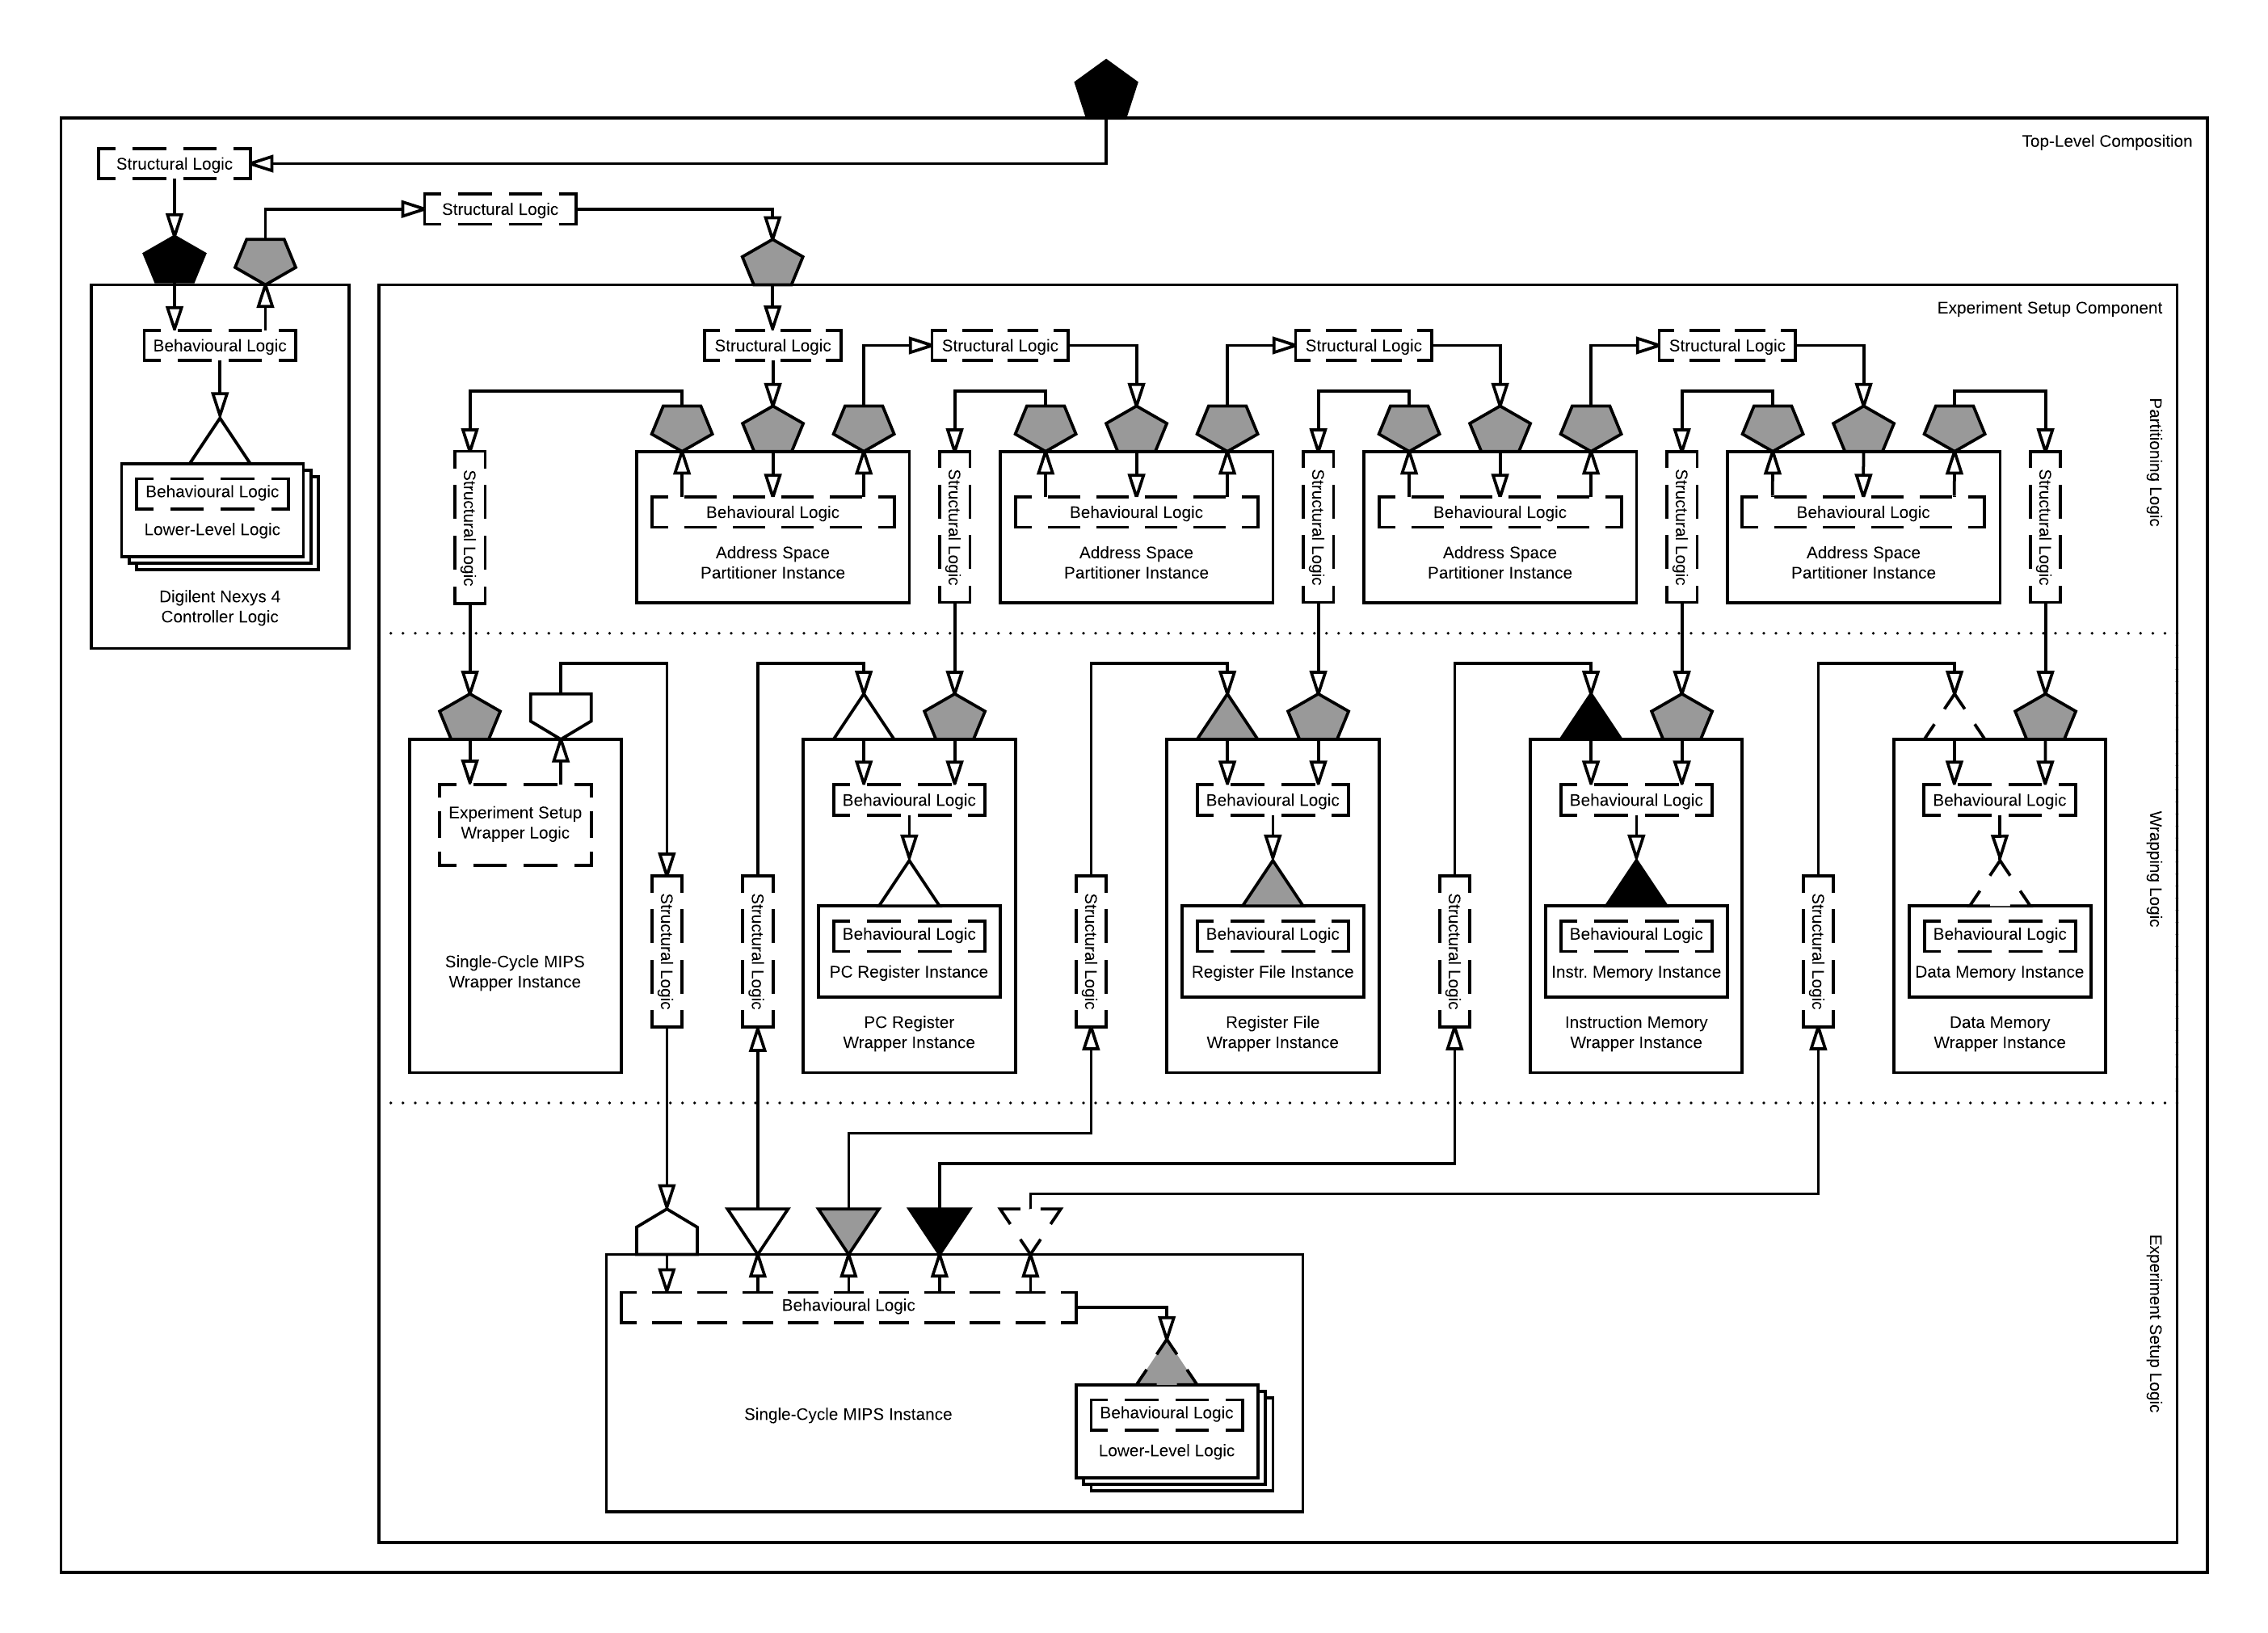
\includegraphics[height=0.95\textwidth,trim=70px 0px 70px 70px, clip=true]{img/mips-wrapped}
    \label{fig:mips-wrapped}
\end{figure}

\end{landscape}

\section{Evaluation}

This article's implementation has been evaluated through functional validation. The original MIPS implementation includes a number of test bench scripts that verify the MIPS' behaviour through the execution of short instruction sequences. These same instruction sequences have been reused in order to validate the behaviour of this article's implementation. The original test bench scripts initialized the instruction memory's contents at compile time and were designed to run in a HDL simulator environment. For this article's implementation however, a different approach has been taken that initialized the instruction memory at runtime while the implementation was executing on a physical FPGA.

A simple preexisting command shell utility was used for interaction with the experiment setup's address space. The test bench instructions could be manually loaded into the MIPS' instruction memory and the program counter could be set to point to the correct position in instruction memory. Through the execution of cycles, these instructions were executed and their effects could be inspected through the read-only debug signals as well as through inspection of the values for the different stateful elements. 




\section{Conclusion}
This article has explored the applicability of the concept of an address space as a means for interaction with an experiment setup's stateful elements. A number of theories and practices have been developed that allow for the projection of such elements on an experiment setup's address space. These theories and practices have been applied to modify a preexisting single-cycle MIPS implementation, allowing for the experiment setup's address space to provide a means of interaction with the different registers and memories that support the MIPS' operation. 

This article's implementation has contributed to the practical applicability of the model as developed in \cite{bos2016model}. The concept of an address space has proven to be a suitable means of interaction with various types of stateful elements. The experiment setup development process has increased terms of complexity and work required. From the experimenter's point of view however, the additional logic introduced for address space projection does not have a negative impact on a transparent means of interaction with experiment setup logic contained within a FPGA development board.

\subsection{Future Work}

\subsubsection{Automated Projection}
The additional work and complexity introduced into the experiment setup development process raises the need for further automation to aid in the development of new experiment setups. The repetitive structures as observed in figure \ref{fig:mips-wrapped} as well as during this article's implementation process suggests that the process of projecting a stateful element on an address space is a candidate for automation. Similar to the previously demonstrated functionality for automated wrapper generation, code generation can play an important in achieving this goal of automated projection of stateful elements. 

While the automated detection of design entity input and output signals is a relatively simple task, the automated detection, externalization and wrapping of stateful elements is considered significantly more challenging. The complexities of HDL modelling languages will likely prove the automated detection of these elements to be especially difficult. One might instead take a hybrid approach in which the process of identification is manually done during the development process, instructing an automated process that generates the logic for address space projection. One approach might be to provide a standard library of stateful components that developers can then use in their experiment implementations. The detection of these standard components can be considered a relatively easy task. Externalization of these standard components can then be achieved through automated refactoring of the HDL design, while the wrapping logic as well as the partitioning logic can be automatically generated based on templates.

\subsubsection{Memory Latencies}
Although mentioned in section \ref{section:async-read}, this article's implementation has not utilized the peripheral SRAM memory device that is available on the Nexys 4 development board. Many FPGA development boards come equipped with large memory devices whose capacity may increase the applicability of the model as a means of hosting experiments setups with large memory requirements. Current work has not included these memory devices in their implementations, but has only included the FPGA's built-in block RAM devices. It is likely that the relatively high latencies of peripheral memory devices can be compensated for through intentional delaying of the experiment setup clock as described in section \ref{section:clock-delay}. 

An underexposed subject in this article however, is the required length of this delay. The block RAM elements used in this article's implementation require a minimum delay of 1 clock cycles if asynchronous read behaviour is desired. However, $n$ cycles of delay are required if $n$ of these asynchronous elements are daisy-chained together in order for one change to propagate through. Including high-latency peripheral memory devices in the design further complicates determining the required duration for delay. The current implementation does not enforce a specific delay in any way. A future implementation might include some form of feedback mechanism for a stateful element to indicate that a new cycle on the experiment setup clock can be initiated. 

\subsubsection{Experimentation Software}
An increased size of the experiment setup's address space description makes it more and more difficult to interact with the experiment setup's address space through simple read and write operations. The address space description of this article's implementation as displayed in table \ref{tbl:address-space} has already proven to be difficult to interact with as the complexity of the actual experiment rises. Loading a large program into the MIPS' instruction memory for example, proves to be impractival trough manual commands. At the time of writing however, work has already started on an improved command line shell application\footnote{https://github.com/fpgaedu/fpgaedu-shell} that aims to tackle these issues. The new software makes use of the provided address space description to aid the experimenter in executing some tasks automatically and prevent manual lookup of addresses. 

% - clock speed
% - feedback logic for long-running memory operations.
% - code generation through preprocessor
% - DRAM
% - PC software is even more essential now the number of elements in the experiment setup address space has increased.

\newpage
\printbibliography

\end{document}
